\mychapter{Credential Relationship Binding Nullifier}

\section{Introduction}

In Chapters 2 and 3, we developed a robust foundation for anonymous credentials, evolving from single-issuer Attribute-Based Anonymous Credentials $(\ABC)$ to the Multi-Issuer Multi-Credential ABC $(\MIMCABC)$ system with identity binding security. $\MIMCABC$ enables users to privately prove that credentials from multiple, mutually distrusting issuers belong to the same identity, a significant advance for applications like federated identity proofs or content credentialing. However, real-world identity systems impose additional requirements that $\MIMCABC$ does not fully address: hierarchical structure and sybil resistance for context-specific credentials.

In practice, credentials often form a natural hierarchy, with foundational identities—such as government-issued IDs or passports—serving as Master Credentials, and dependent credentials—like driver’s licenses, professional certificates, or access rights—acting as Context Credentials. This structure enables efficient revocation: invalidating a Master Credential (e.g., upon employment termination) implicitly revokes all dependent Context Credentials, avoiding the need to track and revoke each individually. Furthermore, regulatory frameworks like KYC/AML demand accountability, requiring systems to prevent sybil attacks where users illegitimately obtain multiple credentials for the same context (e.g., multiple driver’s licenses). 

While MIMC-ABC ensures credentials share a single identity, it lacks mechanisms to enforce this hierarchical dependency or prevent sybil attacks in a privacy-preserving manner, as its identity binding operates agnostically across all credentials without distinguishing their roles or contexts. To meet these practical and regulatory needs, we must extend MIMC-ABC with a cryptographic framework that organizes credentials hierarchically and ensures context-specific uniqueness, all while preserving user anonymity and computational efficiency


\subsection{Problem Statement}

We want to improve MIMC-ABC for real-world use. Our goal is a private credential hierarchy with Sybil resistance. A user has a Master Credential with a secret key $\k$. They also have Context Credentials with unique IDs $\ctx$ (e.g., $\mathcal{H}(\text{"DriverLicense"})$). We need a mechanism that:
\begin{enumerate}
    \item Links each Context Credential to the Master Credential. It uses a unique nullifier $\nul$ from committed values $\k$ and $\ctx$ from different commitments.
    \item Prevents sybil attacks. It prevents multiple nullifiers for the same $(k, \ctx)$ pair.
    \item Verifies nullifier correctness in zero-knowledge. It hides $\k$ and $\ctx$.
\end{enumerate}


Our main challenge is:
\begin{center}
\emph{How do we efficiently generate a verifiable nullifier that proves the binding relationship between two separate credentials without leaking any additional information}
\end{center}


\subsection{Background Work}

Past works tackled hierarchy and sybil resistance in credential systems. None fully balances privacy, efficiency, and flexibility. 
\begin{enumerate}
    \item The UTT anonymous payment system ~\cite{tomescu2022utt} is the closest work, using a registration credential (like a Master Credential) and the coins are also credentials using serial numbers (like Context Credentials) where a coin can only be spent once. UTT uses pairings in their pseudorandom function which we benchmark against and show our speedup.

    \item CanDID~\cite{maram2021candid} defines Master and Context Credentials clearly, but has weakened privacy. It uses mappings between credential public keys in a table, breaking unlinkability. It also relies on an MPC-based PRF for sybil resistance. This adds complexity and overhead, unfit for lightweight use.

    \item Other pairing-based systems, like SyRA~\cite{crites_syra_2024} and S3ID~\cite{rabaninejad_attribute-based_2024}, offer private hierarchies. Yet, they suffer from pairing-related efficiency issues and slower zero-knowledge proofs where we use $\Sigma$-protocols, which are the most efficient zero-knowledge proofs.

    \item Standard Verifiable Random Functions  (VRFs)~\cite{hutchison_verifiable_2005} reveal the user’s public key during verification impacting anonymity and furthermore are constructed with bilinear pairings.

\end{enumerate}

Our MIMC-ABC system (Chapter 3) binds identities efficiently and anonymously but without hierarchy and context-specific sybil resistance. We need a solution that keeps MIMC-ABC’s strengths. It must add a light, private way to handle credential hierarchies and sybil resistance.




\subsection{Contributions}

We advance anonymous credential systems by developing a lightweight, pairing-free Verifiable Random Function (VRF) construction optimized for our use-case of hierarchical credential binding and sybil resistance. Our contributions are threefold:

\begin{enumerate}
        \item \textbf{Pairing-Free VRF in Prime-Order Groups:} We adapt the Dodis-Yampolskiy VRF structure for standard prime-order groups by replacing the proof mechnaism and prove our construction retains the security properties - \emph{pseudorandomness, uniqueness, verifiability} - under the $q$-DHI assumption. (We show the efficiency speedup of this change)

        \item \textbf{Novel $\Sigma$-protocol for Multiplicative Inverse:} We develop a novel zero-knowledge proof protocol to prove that two secret exponents (within a commitment) are the multiplicative inverse of each other. We use this protocol to prove the correctness of the $q$-DHI structure used in the Dodis-Yampolskiy VRF, the technique is a new general technique for $\Sigma$-protocols.
        
        \item \textbf{Credential Relationship Binding Nullifier } We combine our efficient Dodis-Yampolskiy VRF for standard prime-order groups with our Novel $\Sigma$-protocol for multiplicative inverse in addition to a $\Sigma$-proof of additive relation between discrete logarithms to compute our nullifier and show it's 33\% faster for evaluation and 60\% faster for verification than previous constructions while retaining security properties.

\end{enumerate}


\subsection{System Benefits}
Leveraging our technical contributions, the Credential Relationship Binding Nullifier (CRBN) extends the MIMC-ABC system into a complete identity framework with the following benefits:

\begin{enumerate}
    \item Cryptographically binds master credentials (containing key $\k$) to context credentials (with context identifiers $\ctx$) via a verifiable nullifier enabling accountability
    
    \item Enforces sybil resistance for context credentials while retaining privacy by using committed attributes and zero-knowledge proofs
    
    \item Integrates with the efficient $\Sigma$-protocols used throughout the credential system
\end{enumerate}

\subsection*{Chapter Organization}
The remainder of this chapter is organized as follows: Section 4.3 introduces our pairing-free VRF construction in prime-order groups. Section 4.4 presents our zero-knowledge proof protocol for multiplicative inverse relationships. Section 4.5 combines these components to construct the complete Credential Relationship Binding Nullifier (CRBN) system and demonstrates its integration with our identity framework. Finally, Section 4.6 provides a comprehensive performance evaluation comparing our approach to existing techniques.







Pick apart dodis yampolskiy vrf
- the q-BDDHI ensures security of the output which means it must be in a GT element as per the definition $y = e(g,g)^{1/(x+sk)}$ and $\pi = g^{1/(s+sk)}$
- The owner of the function $f$ publishes a public key PK, which can be viewed as a commitment to the function $f$. Something must bind the owner to the function to prove the statement $f(x) = y$. 
- Verify checks $e(g^x \cdot pk, \pi) = e(g,g)$










Redefine Dodis Yampolskiy VRF
1. the assumption (pseudorandomness is indistinguishability coming from the q-DBDHI)



Goal: 

Technical Problems: 
q-DHI is not pseudorandom


















































































\section{Preliminaries}
\subsection{Cryptographic Assumptions}

\begin{definition}[q-DHI Assumption]
Let $\mathbb{G}$ be a cyclic group of prime order $p$ with generator $g$. The $q$-Decisional-Diffie-Hellman Inversion ($q$-DDHI) assumption\cite{mitsunari_new_2002} states that for any PPT adversary $\mathcal{A}$, there exists a negligible function $\negl$ such that:
\[
\Pr\left[ x \sample \Zp^*, \quad \mathcal{A}(g, g^x, g^{x^2}, \ldots, g^{x^q}) = g^{1/x} \right] \leq \negl(\lambda)
\]
where the probability is taken over the random choice of $x$ and the random coins of $\mathcal{A}$. Informally, no $\PPT$ adversary can distinguish between $g^{1/\alpha}$ from a random group element.
\end{definition}

\begin{remark}
The $q$-DHI assumption is equivalent to the $(q+1)$-generalized Diffie-Hellman assumption (GDH) as shown by Boneh and Boyen \cite{kanade_efficient_2004}. This equivalence provides a solid theoretical foundation for the security of our VRF construction.
\end{remark}



\begin{definition}[$q$-BDHI Assumption]
Let $\mathbb{G}$ and $\mathbb{G}_T$ be cyclic groups of prime order $p$ with a bilinear pairing $e: \mathbb{G} \times \mathbb{G} \to \mathbb{G}_T$, and let $g$ be a generator of $\mathbb{G}$. The $q$-Bilinear Diffie-Hellman Inversion ($q$-BDHI) assumption states that for any PPT adversary $\mathcal{A}$, there exists a negligible function $\negl$ such that:
\[
\Pr\left[ x \sample \mathbb{Z}_p^*, \quad \mathcal{A}(g, g^x, g^{x^2}, \ldots, g^{x^q}) = e(g, g)^{1/x} \right] \leq \negl(\lambda)
\]
where the probability is taken over the random choice of $x$ and the random coins of $\mathcal{A}$. Informally, no PPT adversary can compute $e(g, g)^{1/x}$ given $(g, g^x, g^{x^2}, \ldots, g^{x^q})$.
\end{definition}




\subsection{Building Blocks}
We use the Pedersen Commitments from chapter 2, committing to a vector of messages $\cm = \CMCom([\id, \ctx, \exp, \k];\usk) = g_1^\id g_2^\ctx g_3^\exp g_4^\k g^\usk$. Pedersen Commitments are hiding, binding, and position-binding which enforces their position in the vector of messages such that the exponent at one position can't be swapped with another position. 






\begin{definition}[Verifiable Random Function]
We use the definition by \cite{bitansky_verifiable_2020} A Verifiable Random Function (VRF) is a tuple of probabilistic polynomial-time algorithms $(\VRFGen, \VRFEval, \VRFProve, \VRFVerify)$ with an associated message space $\mathcal{X}$, output space $\mathcal{Y}$ and proof space $\Pi$ defined as:
\begin{itemize}
    \item $\VRFGen(1^\lambda) \to (sk, pk)$: Takes a security parameter $\lambda$ and outputs a secret key $sk$ and a public key $pk$.
    
    \item $\VRFEval(sk,x) \to y$: On input $x \in \mathcal{X}$ and secret key $sk$, outputs a value $y \in \mathcal{Y}$.
    
    \item $\VRFProve(sk,x) \to \pi$: On input $x \in \mathcal{X}$ and secret key $sk$, produces a proof $\pi$ that $y$ is consistent with the public key $pk$.
    
    \item $\VRFVerify(pk,x, y, \pi) \to \{0,1\}$: Using the public key $pk$, verifies that $y$ is the correct output for input $x$ with proof $\pi$, returning 1 if valid, 0 otherwise.
\end{itemize}
    
\end{definition}

A $\mathrm{VRF}$ must satisfy three properties:
\begin{itemize}
    \item \textbf{Completeness:} For every security parameter $\lambda \in \mathbb{N}$ and input $x \in \{0,1\}^{n(\lambda)}$:
    \[
    \Pr\left[ \VRFVerify(pk,x, y, \pi) = 1 \ \middle| \ 
    \begin{array}{l}
        (sk, pk) \leftarrow \VRFGen(1^\lambda) \\
        y = \VRFEval(sk,x) \\
        \pi \leftarrow \VRFProve(sk,x)
    \end{array}
    \right] = 1
    \]
    
    \item \textbf{Uniqueness:} For every security parameter $\lambda \in \mathbb{N}$, input $x \in \{0,1\}^{n(\lambda)}$, and arbitrary public key $pk^* \in \{0,1\}^{k(\lambda)}$, there exists at most a single $y \in \{0,1\}^{m(\lambda)}$ for which there exists an accepting proof $\pi$. That is,
    \[
    \text{if} \quad \VRFVerify(pk^*, \pi_0, x, y_0) = \VRFVerify(pk^*, \pi_1, x, y_1) = 1 \quad \text{then} \quad y_0 = y_1
    \]
    
    \item \textbf{Adaptive Indistinguishability:} For any adversary $\mathcal{A}(1^\lambda)$, consider the following game $\mathcal{G}_{\mathcal{A}}^{\text{vrf}}$:
    \begin{enumerate}
        \item The VRF challenger samples $(sk, pk) \leftarrow \VRFGen(1^\lambda)$, and sends $pk$ to $\mathcal{A}$.
        \item $\mathcal{A}$ submits to a challenger evaluation queries $x_1, \ldots, x_Q$, and gets back from the challenger $(y_i, \pi_i), \ldots, (y_Q, \pi_Q)$, where $y_i = \VRFEval(sk, x_i)$, $\pi_i \leftarrow \VRFProve(x_i, sk)$.
        \item At any point, including between evaluation queries, $\mathcal{A}$ may submit a challenge input $x_* \in \{0,1\}^{n(\lambda)}$. The challenger then sets $y_0^* = \VRFEval(sk, x_*)$, $y_1^* \leftarrow \{0,1\}^{m(\lambda)}$, samples $b \leftarrow \{0,1\}$, and sends $y_b^*$ to $\mathcal{A}$. (The adversary $\mathcal{A}$ may then make additional evaluation queries.)
        \item At the end, $\mathcal{A}$ outputs a guess $b'$. The result of the game $\mathcal{G}_{\mathcal{A}}^{\text{vrf}}(\lambda)$ is 1 if $b' = b$, and 0 otherwise.
    \end{enumerate}
    
    We say that $\mathcal{A}$ is \textit{admissible} if in the above game it is always the case that $x_* \not\in \{x_i | i \in [Q]\}$. We require that any polynomial-size admissible adversary wins the game with negligible advantage:
    \[
    \text{Adv}_{\mathcal{A}}^{\text{vrf}} := \left|\Pr\left[\mathcal{G}_{\mathcal{A}}^{\text{vrf}}(\lambda) = 1\right] - \frac{1}{2}\right| \leq \text{negl}(\lambda)
    \]
    
    We say that the VRF satisfies \textit{Selective Indistinguishability} (rather than adaptive) if $\mathcal{A}$ submits the challenge query $x_*$ at the beginning of the game, before getting $pk$ and making any evaluation query.
\end{itemize}

\subsubsection{Zero-Knowledge Proofs}
A zero-knowledge proof (ZKP) enables a prover $\mathcal{P}$ to convince a verifier $\mathcal{V}$ that a statement $x \in L$ holds for a language $L$, without revealing any witness $w$. Formally, an interactive proof system $(\mathcal{P}, \mathcal{V})$ for $L$ satisfies:
\begin{itemize}
    \item \textbf{Completeness}: If $x \in L$, then $\Pr[(\mathcal{P}(w), \mathcal{V})(x) = 1] \geq 1 - \negl(\lambda)$.
    \item \textbf{Soundness}: If $x \notin L$, then for any $\mathcal{P}^*$, $\Pr[(\mathcal{P}^*, \mathcal{V})(x) = 1] \leq \negl(\lambda)$.
    \item \textbf{Zero-Knowledge}: There exists a simulator $\mathcal{S}$ such that for all $x \in L$, the view of any $\mathcal{V}^*$ is computationally indistinguishable from $\mathcal{S}(x)$.
\end{itemize}


\subsubsection{Sigma-Protocols}
A Sigma-protocol is a three-move ZKP where: (1) $\mathcal{P}$ sends a commitment $a$, (2) $\mathcal{V}$ sends a random challenge $e$, and (3) $\mathcal{P}$ responds with $z$. It satisfies:
\begin{itemize}
    \item \textbf{Completeness}: Honest execution accepts with probability 1.
    \item \textbf{Special Soundness}: From two accepting transcripts $(a, e, z)$ and $(a, e', z')$ with $e \neq e'$, a witness $w$ can be extracted.
    \item \textbf{Special Honest-Verifier Zero-Knowledge (SHVZK)}: A simulator can generate transcripts $(a, e, z)$ indistinguishable from real ones for any $e$.
\end{itemize}

















\section{Technical Approach}

\subsection{Starting Point: Dodis-Yampolskiy VRF}

\subsection{Starting Point: Dodis-Yampolskiy VRF}
We begin with the Dodis-Yampolskiy VRF \cite{hutchison_verifiable_2005}, which evaluates $\nul = \tilde{g}^{1/(\k + \ctx)}$ for input $\ctx$ and secret key $\k$. This construction uses bilinear pairings for verification:

\begin{itemize}
    \item $\mathsf{VRF.Gen}(1^\lambda)$: Sample $\k \sample \mathbb{Z}_p^*$, compute $pk = g^\k$. Output $(\k, pk)$.
    \item $\mathsf{VRF.Eval}(\k, \ctx) \to (\nul, \pi)$: Compute $\nul = \tilde{g}^{1/(\k + \ctx)}$ and proof $\pi = e(g, \tilde{g})^{1/(\k + \ctx)}$.
    \item $\mathsf{VRF.Vfy}(pk, \ctx, \nul, \pi) \to \{0, 1\}$: Check if $e(g^{\ctx} \cdot pk, \nul) \stackrel{?}{=} e(g, \tilde{g})$ and $\pi \stackrel{?}{=} e(g, \nul)$.
\end{itemize}

\subsubsection{Informal Security Analysis}
\begin{itemize}
    \item \textbf{Correctness}: The pairing properties ensure that honestly computed $\nul$ and $\pi$ satisfy the verification equations.
    \item \textbf{Uniqueness}: For each $\ctx$, only $\nul = \tilde{g}^{1/(\k + \ctx)}$ satisfies $e(g^{\ctx} \cdot pk, \nul) = e(g, \tilde{g})$.
    \item \textbf{Pseudorandomness}: Under the $q$-DHI assumption, the output $\nul$ appears random to adversaries without knowledge of $\k$.
\end{itemize}

\subsubsection{Limitations}
\begin{enumerate}
    \item It relies on (computationally expensive) bilinear pairings
    \item It operates on public inputs $pk, \ctx$, not allowing for private inputs from commitments
\end{enumerate}

\subsection{Our First Modification: Pairing-Free VRF in Prime-Order Groups}
We adapt the Dodis-Yampolskiy approach to work efficiently in standard prime-order groups without pairings, while maintaining security under the $q$-DHI assumption:

\begin{itemize}
    \item $\mathsf{VRF.Gen}(1^\lambda) \to (\k, pk)$: Sample $\k \sample \mathbb{Z}_p^*$, compute $pk = g^{\k}$. Output $(\k, pk)$.
    \item $\mathsf{VRF.Eval}(\k, \ctx) \to (\nul, \pi)$: Compute $\nul = g^{1/(\k + \ctx)}$ and generate proof $\pi$ using a $\Sigma$-protocol that proves the relation:
    \[
    \mathcal{R} = \zkpok \left\{(pk, \ctx, \nul) (\k) \mid \nul = g^{1/(\k + \ctx)} \quad \wedge \quad pk = g^{\k}  \right\}
    \]
    \item $\mathsf{VRF.Vfy}(pk, \ctx, \nul, \pi) \to \{0,1\}$: Verify the $\Sigma$-protocol proof that $\nul^{\k+\ctx} = g$.
\end{itemize}

\subsubsection{Informal Security Analysis}
\begin{itemize}
    \item \textbf{Correctness}: The $\Sigma$-protocol's completeness ensures that honest provers can convince verifiers.
    \item \textbf{Uniqueness}: The algebraic constraint $\nul^{\k+\ctx} = g$ ensures a unique $\nul$ for each $(\k,\ctx)$ pair.
    \item \textbf{Pseudorandomness}: The $q$-DHI assumption ensures that $g^{1/(\k+\ctx)}$ appears random without knowledge of $\k$.
\end{itemize}

\subsubsection{Limitation}
This modification eliminates pairings but still requires public inputs $(pk, \ctx)$.












\subsection{Our Second Modification: VRF from Committed Inputs}
To support privacy, we extend our construction to operate on committed inputs, hiding both the secret key $\k$ and context identifier $\ctx$:

\begin{itemize}
    \item Input: Commitment $\cm = \CMCom([\k, \ctx]; \usk)$
    \item Output: Nullifier $\nul = g^{1/(\k + \ctx)}$ with zero-knowledge proof $\pi$ for relation:
    \[
    \mathcal{R} = \zkpok \left\{ (\nul, \cm)(\k, \ctx, \usk) \mid \nul = g^{1/(\k + \ctx)} \quad \wedge \quad \cm = g_1^{\k} g_2^{\ctx}g^{\usk}  \right\}
    \]
    \item Verification: The verifier checks the proof $\pi$ without learning $\k$ or $\ctx$.
\end{itemize}

\subsubsection{Informal Security Analysis}
\begin{itemize}
    \item \textbf{Correctness}: The $\Sigma$-protocol's completeness ensures correct nullifiers verify.
    \item \textbf{Uniqueness}: The algebraic structure maintains uniqueness of $\nul$ for each committed $(\k,\ctx)$ pair.
    \item \textbf{Pseudorandomness}: Without knowledge of $\k$, the nullifier remains indistinguishable from random under $q$-DHI.
    \item \textbf{Zero-Knowledge}: The $\Sigma$-protocol reveals nothing about $\k$ or $\ctx$ beyond the fact that $\nul$ is correctly formed.
\end{itemize}

\subsection{Final Construction: VRF from Multiple Committed Inputs}
Our complete construction derives the nullifier from two separate commitments, critical for our anonymous credential system:

\begin{itemize}
    \item Master Credential: $\cmm = \CMCom([\id, \ctx_m, \exp_m, \k]; \usk_m)$ 
    \item Context Credential: $\cmc = \CMCom([\id, \ctx_c, \exp_c]; \usk_c)$
    \item Nullifier: $\nul = g^{1/(\k + \ctx_c)}$
    \item Verification: Zero-knowledge proof for relation:
    \[
    \mathcal{R}_{\mathsf{vrf}} = \zkpok \left\{ 
    \begin{array}{l} 
    (\cmm, \cmc, \nul), \\
    (\id, \ctx_m, \exp_m, \k, \usk_m, \ctx_c, \exp_c, \usk_c) \\
    \end{array} 
    \middle|
    \begin{array}{l}
        \cmm = g_1^{\id}g_2^{\ctx_m}g_3^{\exp_m}g_4^{\k}g^{\usk_m}  \wedge \ctx_m=\texttt{master} \\
        \cmc = g_1^{\id}g_2^{\ctx_c}g_3^{\exp_c}g^{\usk_c} \wedge \ctx_c=\texttt{dmv} \\
        \nul = g^{1/(\k + \ctx_c)}
    \end{array} 
    \right\}
    \]
\end{itemize}

\subsubsection{Informal Security Analysis}
\begin{itemize}
    \item \textbf{Correctness}: Honest provers with valid master and context credentials can generate valid nullifiers.
    \item \textbf{Uniqueness}: Each $(\k,\ctx_c)$ pair produces exactly one nullifier, preventing Sybil attacks.
    \item \textbf{Unlinkability}: Nullifiers for different contexts are unlinkable without knowledge of $\k$.
    \item \textbf{Zero-Knowledge}: The $\Sigma$-protocol reveals nothing about $\id$, $\k$, or any other attributes.
\end{itemize}

This construction enables Sybil resistance while maintaining privacy, as the nullifier deterministically binds a context credential to a master credential without revealing the underlying identity.












\section{Pairing-Free VRF in Prime-Order Groups}

\subsection{Motivation and Design Approach}
Verifiable Random Functions (VRFs) provide verifiable, deterministic, pseudorandom outputs. The Dodis-Yampolskiy VRF \cite{hutchison_verifiable_2005} is particularly well-suited for our credential binding application due to its output formation $y = g^{1/(sk+x)}$. However, the verifiable proof relies on pairings adding computational overhead with each pairing costing approximately 6ms on modern hardware \cite{polgar_anonymous_2025}

Our key insight is that we can replace pairings and generate a proof of correctness with a $\Sigma$-protocol retaining computation in a single group while maintaining all security properties of the original construction and reducing computation costs as shown in our benchmarks (Section 4.6).

\subsubsection{Original Dodis-Yampolskiy Construction}
The Dodis-Yampolskiy VRF is as follows:

\begin{itemize}
    \item $\mathsf{VRF.Gen}(1^\lambda)$: Sample $sk \sample \mathbb{Z}_p^*$, compute $pk = g^{sk} \in \G_1$. Output $(sk, pk)$.
    
    \item $\mathsf{VRF.Eval}(sk, x) \to (\tilde{y}, \pi)$: Compute $\tilde{y} = \tilde{g}^{1/(sk + x)} \in \G_2$ and proof $\pi = e(g, \tilde{g})^{1/(sk + x)} \in \G_T$.
    
    \item $\mathsf{VRF.Vfy}(pk, x, \tilde{y}, \pi) \to \{0, 1\}$: Verify two pairing equations:
    \begin{align}
        e(g^{x} \cdot pk, \tilde{y}) &\stackrel{?}{=} e(g, \tilde{g}) \quad \text{(Equation 1)}\\
        \pi &\stackrel{?}{=} e(g, \tilde{y}) \quad \text{(Equation 2)}
    \end{align}
\end{itemize}

\subsubsection{Analysis}

\paragraph{Output Computation: $\tilde{y} = \tilde{g}^{1/(sk + x)}$}
This is the core VRF output. Under the $q$-DHI assumption, this value appears random to any adversary without knowledge of $sk$, which guarantees the \textbf{pseudorandomness} property.

\paragraph{Verification Equation 1: $e(g^{x} \cdot pk, \tilde{y}) \stackrel{?}{=} e(g, \tilde{g})$}
This equation verifies the algebraic relationship $\tilde{y}^{sk+x} = \tilde{g}$, which is equivalent to $\tilde{y} = \tilde{g}^{1/(sk+x)}$:
\begin{align*}
    e(g^{x} \cdot pk, \tilde{y}) &= e(g^{x} \cdot g^{sk}, \tilde{g}^{1/(sk + x)}) \\
    &= e(g^{sk + x}, \tilde{g}^{1/(sk + x)}) \\
    &= e(g, \tilde{g})^{(sk + x) \cdot 1/(sk + x)} \\
    &= e(g, \tilde{g})
\end{align*}

This verification ensures the \textbf{uniqueness} property: for each $(sk,x)$ pair, only one value $\tilde{y} = \tilde{g}^{1/(sk+x)}$ can satisfy this equation. Any other value would violate the relationship $\tilde{y}^{sk+x} = \tilde{g}$.

\paragraph{Verification Equation 2: $\pi \stackrel{?}{=} e(g, \tilde{y})$}
This equation verifies that the proof $\pi$ is consistent with the output $\tilde{y}$:
\begin{align*}
    \pi &= e(g, \tilde{g})^{1/(sk + x)} \\
    &= e(g, \tilde{g}^{1/(sk + x)}) \\
    &= e(g, \tilde{y})
\end{align*}

This primarily contributes to \textbf{correctness} verification but does not add substantial security beyond Equation 1.

\subsubsection{Key Insight for Our Transformation}

Our key observation is that the critical security properties of the Dodis-Yampolskiy VRF depend on:
\begin{enumerate}
    \item The algebraic structure of the output: $y = g^{1/(sk+x)}$
    \item Verification of the relationship: $y^{sk+x} = g$
    \item The $q$-DHI assumption for pseudorandomness
\end{enumerate}

The pairing operations in the original construction are merely a mechanism to verify the algebraic relationship without revealing $sk$. We can replace these pairing operations with a $\Sigma$-protocol that proves exactly the same relationship: $y^{sk+x} = g$. This maintains all security properties while eliminating expensive pairing computations.









\subsubsection{Analysis of Security Properties}

The Dodis-Yampolskiy VRF construction guarantees three critical security properties through specific components and algebraic relationships:

\subsubsection*{Pseudorandomness}
Output Computation: $\tilde{y} = \tilde{g}^{1/(sk + x)}$ - This is the core VRF output calculated by the holder of the secret key $sk$.
\begin{align*}
    e(g^{x} \cdot pk, \tilde{y}) &= e(g^{x} \cdot g^{sk}, \tilde{g}^{1/(sk + x)}) \\
    &= e(g^{sk + x}, \tilde{g}^{1/(sk + x)}) \\
    &= e(g, \tilde{g})^{(sk + x) \cdot 1/(sk + x)} \\
    &= e(g, \tilde{g})
\end{align*}

Under the $q$-DHI assumption, the value $\tilde{g}^{1/(sk+x)}$ is computationally indistinguishable from a random element in $\mathbb{G}_2$ to any party without knowledge of $sk$, even after seeing VRF outputs for other inputs.


\subsubsection*{Uniqueness}
 Verification Equation 1: $e(g^{x} \cdot pk, \tilde{y}) \stackrel{?}{=} e(g, \tilde{g})$ verifies that $\tilde{y}^{sk+x} = \tilde{g}$ without requiring knowledge of $sk$

This equation ensures that for each $(sk,x)$ pair, only one value $\tilde{y} = \tilde{g}^{1/(sk+x)}$ can satisfy the verification. Any alternative value would fail to satisfy the pairing equation, making it impossible to generate two different valid outputs for the same input.












\begin{itemize}
    \item \textbf{Pseudorandomness:} Under the $q$-DHI assumption, the value $\tilde{g}^{1/(sk+x)}$ is computationally indistinguishable from a random element in $\mathbb{G}_2$ to any party without knowledge of $sk$, even after seeing VRF outputs for other inputs.
\end{itemize}

\paragraph{Output Computation: $\tilde{y} = \tilde{g}^{1/(sk + x)}$}
This is the core VRF output calculated by the holder of the secret key $sk$.
\begin{align*}
    e(g^{x} \cdot pk, \tilde{y}) &= e(g^{x} \cdot g^{sk}, \tilde{g}^{1/(sk + x)}) \\
    &= e(g^{sk + x}, \tilde{g}^{1/(sk + x)}) \\
    &= e(g, \tilde{g})^{(sk + x) \cdot 1/(sk + x)} \\
    &= e(g, \tilde{g})
\end{align*}

\begin{itemize}
    \item \textbf{Pseudorandomness:} Under the $q$-DHI assumption, the value $\tilde{g}^{1/(sk+x)}$ is computationally indistinguishable from a random element in $\mathbb{G}_2$ to any party without knowledge of $sk$, even after seeing VRF outputs for other inputs.
\end{itemize}

\paragraph{Verification Equation 1: $e(g^{x} \cdot pk, \tilde{y}) \stackrel{?}{=} e(g, \tilde{g})$}
This equation verifies that $\tilde{y}^{sk+x} = \tilde{g}$ without requiring knowledge of $sk$.

\begin{itemize}
    \item \textbf{Uniqueness:} This equation ensures that for each $(sk,x)$ pair, only one value $\tilde{y} = \tilde{g}^{1/(sk+x)}$ can satisfy the verification. Any alternative value would fail to satisfy the pairing equation, making it impossible to generate two different valid outputs for the same input.
\end{itemize}

\paragraph{Verification Equation 2: $\pi \stackrel{?}{=} e(g, \tilde{y})$}
This equation verifies the consistency of the proof $\pi$ with the output $\tilde{y}$.
\begin{align*}
    \pi &= e(g, \tilde{g})^{1/(sk + x)} \\
    &= e(g, \tilde{g}^{1/(sk + x)}) \\
    &= e(g, \tilde{y})
\end{align*}

\begin{itemize}
    \item \textbf{Correctness:} This verification ensures that an honest evaluator who knows $sk$ can always produce outputs and proofs that pass verification.
\end{itemize}

\subsubsection*{Key Security Requirements}
Our analysis identifies three essential requirements that must be preserved in any transformation of the Dodis-Yampolskiy VRF:

\begin{enumerate}
    \item \textbf{Output Structure:} Maintain the form $y = g^{1/(sk+x)}$ to preserve pseudorandomness under the $q$-DHI assumption.
    
    \item \textbf{Algebraic Verification:} Ensure verification confirms the relationship $y^{sk+x} = g$ without revealing $sk$.
    
    \item \textbf{Proof Consistency:} Provide a means to verify that proofs are consistent with outputs and cannot be forged.
\end{enumerate}

The pairing operations in the original construction serve primarily as a mechanism to verify these algebraic relationships without revealing $sk$. By replacing these pairings with a carefully designed $\Sigma$-protocol that proves exactly the same relationships, we can maintain all security properties while eliminating computationally expensive pairing operations.



















\subsubsection{Analysis of Security Properties}
The Dodis-Yampolskiy VRF construction guarantees three critical security properties. We analyze each property and identify which components and algebraic relationships ensure them:

\paragraph{Pseudorandomness}
The output $\tilde{y} = \tilde{g}^{1/(sk + x)}$ appears random to any observer without knowledge of $sk$. 

Under the $q$-DHI assumption, given $(g, g^{sk}, g^{(sk)^2}, ..., g^{(sk)^q})$ for any polynomial $q$, computing $g^{1/(sk+x)}$ for any $x$ not previously queried is computationally infeasible. The VRF inherits this property directly from its output structure, making the value $\tilde{g}^{1/(sk+x)}$ indistinguishable from a random element in $\mathbb{G}_2$.

Critically, the verification equations themselves do not weaken this pseudorandomness guarantee, as they only confirm algebraic relationships without revealing additional information about $sk$.

\paragraph{Uniqueness}
Verification Equation 1: $e(g^{x} \cdot pk, \tilde{y}) \stackrel{?}{=} e(g, \tilde{g})$ enforces that only one valid output can exist for each input.

This equation verifies the algebraic relationship $\tilde{y}^{sk+x} = \tilde{g}$ without requiring knowledge of $sk$:
\begin{align*}
    e(g^{x} \cdot pk, \tilde{y}) &= e(g^{x} \cdot g^{sk}, \tilde{g}^{1/(sk + x)}) \\
    &= e(g^{sk + x}, \tilde{g}^{1/(sk + x)}) \\
    &= e(g, \tilde{g})^{(sk + x) \cdot 1/(sk + x)} \\
    &= e(g, \tilde{g})
\end{align*}

This uniqueness guarantee is crucial: for each $(sk,x)$ pair, only the value $\tilde{y} = \tilde{g}^{1/(sk+x)}$ can satisfy this equation. Any attempt to forge a different output $\tilde{y}'$ would require solving the discrete logarithm problem in $\mathbb{G}_2$.

\paragraph{Correctness}
The combination of both verification equations ensures that honestly generated outputs and proofs will always verify:

1. Verification Equation 1: $e(g^{x} \cdot pk, \tilde{y}) \stackrel{?}{=} e(g, \tilde{g})$ ensures output correctness

2. Verification Equation 2: $\pi \stackrel{?}{=} e(g, \tilde{y})$ ensures proof consistency:
\begin{align*}
    \pi &= e(g, \tilde{g})^{1/(sk + x)} \\
    &= e(g, \tilde{g}^{1/(sk + x)}) \\
    &= e(g, \tilde{y})
\end{align*}

Together, these equations guarantee that an honest evaluator with knowledge of $sk$ will always produce outputs and proofs that pass verification.

\paragraph{Key Requirements for Transformation}
Based on this analysis, any transformation of the Dodis-Yampolskiy VRF must preserve:

\begin{enumerate}
    \item The output structure $y = g^{1/(sk+x)}$ to maintain pseudorandomness under $q$-DHI
    
    \item A verification mechanism that confirms $y^{sk+x} = g$ without revealing $sk$ to ensure uniqueness
    
    \item A means to verify proof consistency with outputs to guarantee correctness
\end{enumerate}

In our pairing-free construction, we will replace the pairing-based verification with a $\Sigma$-protocol that proves exactly these same algebraic relationships while eliminating expensive pairing computations.

































\subsection{Construction}
Our VRF operates in a prime-order group $\mathbb{G}$ of order $p$ with generator $g$. Define the message space $\setX = \mathbb{Z}_p$, output space $\setY = \mathbb{G}$, and proof space $\Pi = \mathbb{G} \times \mathbb{G} \times \mathbb{Z}_p$. 


\begin{itemize}
    \item $\mathsf{VRF.Gen}(1^\lambda) \to (sk, pk)$:  
    Sample $sk \sample \mathbb{Z}_p^*$, compute $pk = g^{sk}$, and output $(sk, pk)$.
    
    \item $\mathsf{VRF.Eval}(sk, x) \to (y, \pi)$:  
    Compute $y = g^{1/(sk + x)}$ and generate proof $\pi$ using the $\Sigma$-protocol described below.
    
    \item $\mathsf{VRF.Vfy}(pk, x, y, \pi) \to \{0,1\}$:
    Verify that $y$ is correctly formed using the $\Sigma$-protocol verification.
\end{itemize}


\subsection{Proof Protocol}
To prove that $y = g^{1/(sk+x)}$ without revealing $sk$, we use a $\Sigma$-protocol that demonstrates knowledge of $sk$ such that $pk = g^{sk}$ and $y^{sk+x} = g$. The protocol operates as follows:

\begin{protocol}{$\pi$ for VRF Prime Order Group}{}\label{pok-vrf-prime-order-group}
\textbf{Relation: }
\[
\mathcal{R} = \{(pk, x, y), (sk) \mid pk = g^{sk} \wedge y^{sk+x} = g\}
\]
\textbf{Common Input:} Generator $g \in \G$, public elements $pk, y \in \G$ and VRF input $x \in \Z_q$\\
\textbf{Prover Input:} Witness $(sk)$ such that: $y = g^{1/(sk + x)}$
\begin{enumerate}
    \item \textbf{Commitment:} Prover samples $r \sample \Z_q$, computes 
    \[
    T_1 = g^r \qquad T_2 = y^r
    \]
    Sends $(T_1, T_2)$ to verifier.
    
    \item \textbf{Challenge:} Verifier samples $c \sample \mathbb{Z}_q$ and sends to prover.
    
    \item \textbf{Response:} Prover computes:
    \[
    z = r + c \cdot (sk + x)
    \]
    Sends $z$ to verifier
    
    \item \textbf{Verification:} Verifier computes $C = pk \cdot g^x \quad =(g^{sk + x})$ and checks:
    \[
    T_1 \cdot C^c \stackrel{?}{=} g^z \qquad T_2 \cdot g^c \stackrel{?}{=} y^z
    \]
 
\end{enumerate}
\end{protocol}

\subsection{Security Analysis}
Our construction preserves the three essential VRF properties - correctness, uniqueness, and pseudorandomness - under the $q$-DHI assumption.


This construction satisfies the VRF properties - correctness, uniqueness, and pseudorandomness under the under the $q$-DHI assumption. Note that we use a public key $pk$ and VRF input $x$ which are both public. 

\subsubsection{Comparison to Dodis-Yampolskiy VRF}
The Dodis-Yampolskiy VRF also evaluates $y = g^{1/(sk + x)}$, but relies on a bilinear group for the proof $\pi$ using a pairing check: $e(y, pk \cdot g^x) = e(g, g)$, which is computationally heavy. Our construction sticks to the prime-order group, proves $y^{sk + x} = g$ with a $\Sigma$-protocol.


\subsection{Security Analysis}
Our construction preserves the three essential VRF properties - correctness, uniqueness, and pseudorandomness - under the same $q$-DHI assumption as the original Dodis-Yampolskiy VRF.

\subsubsection*{Correctness}
An honest prover computing $y = g^{1/(sk+x)}$ can always convince the verifier by executing the $\Sigma$-protocol. This follows from the following equalities:
$$g^z = g^{r + c(sk+x)} = g^r \cdot (g^{sk} \cdot g^x)^c = T_1 \cdot C^c$$
$$y^z = y^{r + c(sk+x)} = y^r \cdot y^{sk+x} = y^r \cdot g = T_2 \cdot g^c$$

\subsubsection*{Uniqueness}
For each $(sk,x)$ pair, only one valid output $y$ can satisfy the verification equation $y^{sk+x} = g$, namely $y = g^{1/(sk+x)}$. Any attempt to provide a different output would fail the verification protocol.

\subsubsection*{Pseudorandomness}
Under the $q$-DHI assumption, $g^{1/(sk+x)}$ is indistinguishable from random for any adversary without knowledge of $sk$. Our verification protocol reveals no additional information about $sk$ beyond what was already leaked in the original Dodis-Yampolskiy construction, preserving the pseudorandomness property.
















\section{Pairing-Free VRF in Prime-Order Groups}

\subsection{From Pairings to Sigma Protocols: A Transformation}

The Dodis-Yampolskiy VRF \cite{hutchison_verifiable_2005} evaluates $y = g^{1/(sk+x)}$ and verifies correctness through a bilinear pairing check:
\begin{equation}
e(y, pk \cdot g^x) = e(g, g)
\end{equation}

This equation verifies that $y^{sk+x} = g$ without revealing $sk$, as we can expand:
\begin{align}
e(g^{1/(sk+x)}, g^{sk} \cdot g^x) &= e(g, g)\\
e(g^{1/(sk+x)}, g^{sk+x}) &= e(g, g)\\
e(g, g)^{1/(sk+x) \cdot (sk+x)} &= e(g, g)\\
e(g, g)^1 &= e(g, g)
\end{align}

Our key insight is that we can directly prove the relationship $y^{sk+x} = g$ using a $\Sigma$-protocol without relying on pairings. This provides the same security guarantees while significantly reducing computational costs, as pairing operations are typically 5-10× more expensive than standard group operations.

\subsection{Construction}
[Include your VRF construction as before]

\subsection{Proof Protocol}
Our $\Sigma$-protocol proves exactly the same relation that the pairing check verifies in Dodis-Yampolskiy: namely, that the prover knows $sk$ such that $pk = g^{sk}$ and $y^{sk+x} = g$.

[Include your protocol steps as before]

\subsection{Security Analysis}

\subsubsection{Equivalence to Dodis-Yampolskiy Verification}
We first establish that our verification mechanism is equivalent to the pairing-based check in Dodis-Yampolskiy. Both approaches verify that $y = g^{1/(sk+x)}$:

\begin{itemize}
    \item \textbf{Dodis-Yampolskiy}: Verifies through $e(y, pk \cdot g^x) = e(g, g)$, which holds if and only if $y = g^{1/(sk+x)}$.
    
    \item \textbf{Our approach}: The $\Sigma$-protocol verification equations $g^z = T_1 \cdot C^c$ and $y^z = T_2 \cdot g^c$ together ensure that $y^{sk+x} = g$, which holds if and only if $y = g^{1/(sk+x)}$.
\end{itemize}

This equivalence ensures that our construction preserves all security properties of the original VRF while eliminating pairing operations.

\subsubsection{$\Sigma$-Protocol Security}
Our protocol satisfies the three required properties of a secure $\Sigma$-protocol:

\textbf{Completeness:} An honest prover with knowledge of $sk$ always succeeds. For $z = r + c(sk+x)$:
\begin{align}
g^z &= g^{r + c(sk+x)} = g^r \cdot (g^{sk} \cdot g^x)^c = T_1 \cdot C^c\\
y^z &= y^{r + c(sk+x)} = y^r \cdot (y^{sk+x}) = y^r \cdot g = T_2 \cdot g^c
\end{align}

\textbf{Special Soundness:} Given two accepting transcripts $(T_1, T_2, c, z)$ and $(T_1, T_2, c', z')$ where $c \neq c'$, we can extract $sk$ as follows:
\begin{align}
g^z &= T_1 \cdot C^c \quad \text{and} \quad g^{z'} = T_1 \cdot C^{c'}\\
\Rightarrow g^{z-z'} &= C^{c-c'} = (pk \cdot g^x)^{c-c'}\\
\Rightarrow g^{z-z'} &= g^{(sk+x)(c-c')}\\
\Rightarrow z-z' &= (sk+x)(c-c')\\
\Rightarrow sk &= \frac{z-z'}{c-c'} - x
\end{align}

Thus, we can extract the secret key $sk$, confirming that the prover must know $sk$ to convince the verifier.

\textbf{Zero-Knowledge:} We can simulate accepting transcripts without knowing $sk$:
\begin{enumerate}
    \item Sample $z \sample \mathbb{Z}_p$ and $c \sample \mathbb{Z}_p$ uniformly
    \item Compute $T_1 = g^z \cdot (pk \cdot g^x)^{-c}$ and $T_2 = y^z \cdot g^{-c}$
    \item Output $(T_1, T_2, c, z)$
\end{enumerate}
This simulation is perfectly indistinguishable from real protocol transcripts.

\subsubsection{VRF Security Properties}
Building on this $\Sigma$-protocol foundation, our VRF preserves all three essential properties:

\textbf{Correctness:} [As before]

\textbf{Uniqueness:} [As before]

\textbf{Pseudorandomness:} The security reduction to the $q$-DHI assumption follows exactly as in Dodis-Yampolskiy. An adversary distinguishing VRF outputs from random would solve the $q$-DHI problem. Our verification mechanism reveals exactly the same information as the pairing check, maintaining the same pseudorandomness guarantee.




























































\clearpage
\section{Construction 2.0. Proving Committed Multiplicative Inverse}


- mention the benefit of the pairing here - it effectively multiplies the two together which isn't possible with standard group elements - that's the challenge we had to get through.

Let $G$ be a cyclic group of prime order $q$, with generators $g_1, g \in G$. Assume the discrete logarithm problem (DLP) is hard in $G$, and the discrete log of $g_1$ with respect to $g$ is unknown.
The prover aims to prove in zero-knowledge that there exists $m \in \mathbb{Z}_q^*$ such that $m \cdot x = 1 \mod q$, where $x = \frac{1}{m}$, given commitments to $m$ and $x$.

\begin{protocol}{Proving Committed Multiplicative Inverse}{committed-multiplicative-inverse}\label{pok-committed-multiplicative-inverse}
\textbf{Common Input:} Group generators $g_1, g \in \mathbb{G}$, and commitments $\cm_1, \cm_2, \cm_3, \cm_4 \in \mathbb{G}$\\
\textbf{Prover Input:} Witness $(m, x, \usk_1, \usk_2, \usk_3, \usk_4)$ such that:
    \begin{align*}
        \cm_1 &= g_1^m g^{\usk_1}     &    \cm_2 &= g_1^x g^{\usk_2}  &   \cm_3 &= \cm_2^m g^{\usk_3} & \cm_4 &= g^{\usk_4}\\
         x &= \frac{1}{m}     &   \usk_4 &= \usk_3 + m \usk_2 & \frac{\cm_3}{\cm_4} &= g_1
    \end{align*}
\begin{enumerate}
    \item \textbf{Commitment:} Prover samples random blinding factors from $\Z_q$:
       \[
        a_x \quad \text{ for } \quad x \in \{\ m, x, \usk_1, \usk_2, \usk_3, \usk_4\} \in \Z_q
        \]
    \textbf{Computes}:
    \begin{align*}
        T_1 &\gets g_1^{a_m} g^{a_{\usk_1}}  &   T_2 &\gets g_1^{a_x} g^{a_{\usk_2}}     &   T_3 &\gets \cm_2^{a_m} g^{a_{\usk_3}} & T_4 &\gets g^{a_{\usk_4}}
    \end{align*}
    Sends $(T_1, T_2, T_3, T_4)$ to verifier.
    
    \item \textbf{Challenge:} Verifier samples $c \sample \mathbb{Z}_q$ and sends to prover.
    
    \item \textbf{Response:} Prover computes:
    \[
    z_x = a_x + c \cdot x \quad \text{ for } \quad x \in \{\ m, x, \usk_1, \usk_2, \usk_3, \usk_4\} 
    \]
    Sends $(z_m, z_x, z_{\usk_1}, z_{\usk_2}, z_{\usk_3}, z_{\usk_4})$ to verifier.
    
    \item \textbf{Verification:} Verifier checks:
    \begin{align*}
         T_1 \cdot \cm_1^c &\stackrel{?}{=}  g_1^{z_1} g^{z_2}
        & 
         T_2 \cdot \cm_2^c &\stackrel{?}{=}  g_1^{z_3} g^{z_4}\\
        T_3 \cdot \cm_3^c &\stackrel{?}{=} \cm_2^{z_1} g^{z_5}
        &
        T_4 \cdot \cm_4^c &\stackrel{?}{=}  g^{z_6} 
        &
        \frac{\cm_3}{\cm_4} &\stackrel{?}{=} g_1
    \end{align*}
\end{enumerate}
\end{protocol}

\subsubsection*{Completeness}:
We show that if the prover follows the protocol honestly, all verification equations will be satisfied.

\begin{enumerate}
    \item The first two verification equations ($T_1 \cdot \cm_1^c \stackrel{?}{=} g_1^{z_m} g^{z_{\usk_1}}$, $T_2 \cdot \cm_2^c \stackrel{?}{=} g_1^{z_x} g^{z_{\usk_2}}$) are simple Schnorr proofs of exponents which we will not expand 
        
    \item Third verification equation: $T_3 \cdot \cm_3^c \stackrel{?}{=} \cm_2^{z_m} g^{z_{\usk_3}}$
    \begin{align*}
        T_3 \cdot \cm_3^c &= \cm_2^{a_m} g^{a_{\usk_3}} \cdot (\cm_2^m g^{\usk_3})^c \\
        &= \cm_2^{a_m} g^{a_{\usk_3}} \cdot \cm_2^{m \cdot c} g^{\usk_3 \cdot c} \\
        &= \cm_2^{a_m + m \cdot c} g^{a_{\usk_3} + \usk_3 \cdot c} \\
        &= \cm_2^{z_m} g^{z_{\usk_3}}
    \end{align*}
    
    \item Fourth verification equation: $T_4 \cdot \cm_4^c \stackrel{?}{=} g^{z_{\usk_4}}$
    \begin{align*}
        T_4 \cdot \cm_4^c &= g^{a_{\usk_4}} \cdot (g^{\usk_4})^c \\
        &= g^{a_{\usk_4}} \cdot g^{\usk_4 \cdot c} \\
        &= g^{a_{\usk_4} + \usk_4 \cdot c} \\
        &= g^{z_{\usk_4}}
    \end{align*}
    
    \item Fifth verification equation: $\frac{\cm_3}{\cm_4} \stackrel{?}{=} g_1$
    
    Using the relations $x = \frac{1}{m}$ and $\usk_4 = \usk_3 + m \cdot \usk_2$:
    \begin{align*}
        \cm_3 &= \cm_2^m g^{\usk_3} \\
        &= (g_1^x g^{\usk_2})^m g^{\usk_3} \\
        &= g_1^{x \cdot m} g^{\usk_2 \cdot m} g^{\usk_3} \\
        &= g_1^{\frac{1}{m} \cdot m} g^{\usk_2 \cdot m + \usk_3} \\
        &= g_1 g^{\usk_3 + m \cdot \usk_2} \\
        &= g_1 g^{\usk_4} \\
        &= g_1 \cdot \cm_4
    \end{align*}
    
    Therefore:
    \begin{align*}
        \frac{\cm_3}{\cm_4} = \frac{g_1 \cdot \cm_4}{\cm_4} = g_1
    \end{align*}
\end{enumerate}

Since all verification equations are satisfied when the prover follows the protocol, we conclude that our sigma protocol satisfies the completeness property.


\subsubsection*{Soundness}
We prove the special soundness property by demonstrating that given two accepting transcripts with identical first messages but different challenges, we can extract a valid witness satisfying all relations required by the protocol.

Let $(T_1, T_2, T_3, T_4, c, z_m, z_x, z_{\usk_1}, z_{\usk_2}, z_{\usk_3}, z_{\usk_4})$ and $(T_1, T_2, T_3, T_4, c', z'_m, z'_x, z'_{\usk_1}, z'_{\usk_2}, z'_{\usk_3}, z'_{\usk_4})$ be two accepting transcripts with $c \neq c'$.

\begin{enumerate}
    \item \textbf{Witness extraction:}
    
    Following the standard extraction technique for sigma protocols, we compute each witness component:
    \begin{align}
    m &= \frac{z_m - z'_m}{c - c'} & x &= \frac{z_x - z'_x}{c - c'} \\
    \usk_1 &= \frac{z_{\usk_1} - z'_{\usk_1}}{c - c'} & \usk_2 &= \frac{z_{\usk_2} - z'_{\usk_2}}{c - c'} \\
    \usk_3 &= \frac{z_{\usk_3} - z'_{\usk_3}}{c - c'} & \usk_4 &= \frac{z_{\usk_4} - z'_{\usk_4}}{c - c'}
    \end{align}
    
    These extracted values are guaranteed to be consistent with the protocol's verification equations precisely because both transcripts are accepting.
    
    \item \textbf{Verification of commitment relations:}
    
    We first show that the extracted witness satisfies $\cm_1 = g_1^m g^{\usk_1}$. From the acceptance of both transcripts, we have:
    \begin{align}
        T_1 \cdot \cm_1^c &= g_1^{z_m} g^{z_{\usk_1}} \\
        T_1 \cdot \cm_1^{c'} &= g_1^{z'_m} g^{z'_{\usk_1}}
    \end{align}
    
    Dividing these equations and substituting our extracted values:
    \begin{align}
        \cm_1^{c-c'} &= g_1^{z_m-z'_m} g^{z_{\usk_1}-z'_{\usk_1}} \\
        &= g_1^{m(c-c')} g^{\usk_1(c-c')} \\
        \Rightarrow \cm_1 &= g_1^m g^{\usk_1}
    \end{align}
    
    Using identical extraction and verification techniques with the corresponding verification equations, we establish that:
    \begin{align}
        \cm_2 &= g_1^x g^{\usk_2} \\
        \cm_3 &= \cm_2^m g^{\usk_3} \\
        \cm_4 &= g^{\usk_4}
    \end{align}
    
    \item \textbf{Verification of the multiplicative inverse relation ($x = \frac{1}{m}$):}
    
    The core cryptographic property enforced by our protocol is the multiplicative inverse relationship between $m$ and $x$. This is where the protocol's security guarantee is ultimately derived from. We verify this relationship using the final verification equation $\frac{\cm_3}{\cm_4} = g_1$.
    
    Substituting our extracted witness values:
    \begin{align}
        \frac{\cm_3}{\cm_4} &= g_1 \\
        \frac{\cm_2^m g^{\usk_3}}{g^{\usk_4}} &= g_1 \\
        \cm_2^m g^{\usk_3 - \usk_4} &= g_1
    \end{align}
    
    Further substituting $\cm_2 = g_1^x g^{\usk_2}$:
    \begin{align}
        (g_1^x g^{\usk_2})^m g^{\usk_3 - \usk_4} &= g_1 \\
        g_1^{x \cdot m} g^{m \cdot \usk_2 + \usk_3 - \usk_4} &= g_1
    \end{align}
    
    In the generic group model, this equation can only hold if:
    \begin{align}
        x \cdot m &= 1 \\
        m \cdot \usk_2 + \usk_3 - \usk_4 &= 0
    \end{align}
    
    These equations immediately give us the two critical relations:
    \begin{align}
        x &= \frac{1}{m} \\
        \usk_4 &= \usk_3 + m\usk_2
    \end{align}
    
    The first relation confirms that our protocol successfully enforces the multiplicative inverse relationship between $m$ and $x$. The second relation verifies the consistency of the randomizers across the commitments, ensuring that no malicious prover can construct valid-looking commitments without knowing values that satisfy all required relations.
\end{enumerate}

We have thus demonstrated that our extractor obtains a complete and valid witness $(m, x, \usk_1, \usk_2, \usk_3, \usk_4)$ satisfying all relations in the statement, establishing the special soundness property of our sigma protocol. This ensures that no prover can successfully convince a verifier without knowledge of values satisfying the multiplicative inverse relationship $x = \frac{1}{m}$ and the associated consistency requirements.

\subsubsection*{Zero-Knowledge}
We prove the honest-verifier zero-knowledge property by presenting a simulator that produces transcripts indistinguishable from real protocol executions without knowing any witness.

\begin{enumerate}
    \item \textbf{Simulator Construction:}
    
    Given public input $(g_1, g, \cm_1, \cm_2, \cm_3, \cm_4)$ and any challenge $c \in \mathbb{Z}_q$, our simulator:
    
    \begin{itemize}
        \item Samples $z_m, z_x, z_{\usk_1}, z_{\usk_2}, z_{\usk_3}, z_{\usk_4} \sample \mathbb{Z}_q$ uniformly at random
        
        \item Computes the first message by working backwards from the verification equations:
        \begin{align}
            T_1 &\gets g_1^{z_m} g^{z_{\usk_1}} \cdot \cm_1^{-c} \\
            T_2 &\gets g_1^{z_x} g^{z_{\usk_2}} \cdot \cm_2^{-c} \\
            T_3 &\gets \cm_2^{z_m} g^{z_{\usk_3}} \cdot \cm_3^{-c} \\
            T_4 &\gets g^{z_{\usk_4}} \cdot \cm_4^{-c}
        \end{align}
        
        \item Outputs the transcript $(T_1, T_2, T_3, T_4, c, z_m, z_x, z_{\usk_1}, z_{\usk_2}, z_{\usk_3}, z_{\usk_4})$
    \end{itemize}
    
    \item \textbf{Perfect Indistinguishability:}
    
    In a real protocol execution with an honest prover, the responses have the form $z_x = a_x + c \cdot x$ where $a_x$ are uniformly random values. Since $a_x \sample \mathbb{Z}_q$ and addition with $c \cdot x$ is a permutation over $\mathbb{Z}_q$, the distribution of real responses is uniform over $\mathbb{Z}_q$.
    
    The simulator directly samples responses uniformly from $\mathbb{Z}_q$, matching this distribution exactly. Given these responses and the challenge $c$, the first message components $T_i$ are uniquely determined by the verification equations in both real and simulated cases.
    
    Consequently, the joint distribution of $(T_1, T_2, T_3, T_4, c, z_m, z_x, z_{\usk_1}, z_{\usk_2}, z_{\usk_3}, z_{\usk_4})$ is identical for both the simulator and the honest protocol.
\end{enumerate}

This construction demonstrates that our protocol satisfies perfect honest-verifier zero-knowledge. Notably, the simulator succeeds without requiring knowledge of the critical multiplicative inverse relationship $x = \frac{1}{m}$ or any other witness values, confirming that the protocol reveals no information about these secret values beyond what is already implied by the statement being proven.








































\clearpage
OLD WORK AND NOTES







\subsection{Construction}
During verification, the user proves in zero-knowledge that they possess a valid master credential with VRF key $\k$, a context credential with a specific $\ctx$ value and the nullifier $\nul$ is correctly formed by using a secret $\k$ in $\credm$ and $\ctx$ in $\credc$. 

\begin{equation}
\nul = g^{1/(\k + \ctx)} \in \G
\end{equation}

\subsection{Integration with Identity System}


\begin{figure}
        \begin{pchstack}[boxed, center, space=4em]
            \begin{pcvstack}
                \procedure[space=auto]{Passport}{%
                \id: 12345, \\
                \ctx: "master", \\
                \exp: "10/11/2026" \\
                \k: 54321
                }
            \end{pcvstack}
            \pcvspace
            \begin{pcvstack}
                \procedure[space=auto]{Driver License}{%
                 \id: 12345, \\
                 \ctx: "DMV", \\
                 \exp: "10/11/2028"
                }
            \end{pcvstack}
            \begin{pcvstack}
                \procedure[space=auto]{Nullifier}{%
                 \textsf{n} = 1/(\k + "DMV") \\
                 \nul = g^{\textsf{n}}
                }
            \end{pcvstack}
        \end{pchstack}
    \caption{Example Credential and Nullifier for context DMV}
    \label{fig:two-creds}
\end{figure}


\[
    \mathcal{R}_{\mathsf{vrf}} = \zkpok \left\{ 
    \begin{array}{l} 
    (\cmm, \cmc, \mathsf{N}), (\id, \ctx, , \exp, \k, r_1, r_2) \\
    \end{array} 
    \middle|
    \begin{array}{l}
        \cmm = g_1^{\id}g_2^{\ctx}g_3^{\exp}g_4^{\k}g^{r_1}  \wedge \ctx="master" \\
        \cmc = g_1^{\id}g_2^{\ctx}g_3^{\exp}g^{r_2} \wedge \ctx="DMV" \\
        \nul = g^{1/(k + \ctx)}
    \end{array} 
    \right\}
\]
    



\section{CRBN Instantiation for Identity System}

\begin{protocol}{CRBN Instantiation Two Commitments}{}\label{crbn-instantiation}
\textbf{Common Input:} Group generators $g_1, g_2, g_3, g_4, g_5, g \in \mathbb{G}$, and commitments $\cm_1, \cm_2, \cm_3, \cm_4, \cm_5, \cm_6 \in \mathbb{G}$\\
\textbf{Prover Input:} Witness $(\id, \k, \ctx, r_1, r_2, r_3, r_4, r_5, \textsf{n}, r_6)$ such that:
    \begin{align*}
        \cm_1 &= g_1^{\id} g_2^{\k} g^{r_1}     &    \cm_2 &= g_1^{\id} g_3^{\ctx} g^{r_2}  &   \cm_3 &= g_4^{\k + \ctx} g^{r_3}\\
        \cm_4 &= g_5^{1/(\k + \ctx)} g^{r_4}   &   \cm_5 &= \cm_3^{1/(\k + \ctx)} g^{r_5}     &   \cm_6 &= g^{r_6} \\
       r_6 &= r_3 \cdot \frac{1}{\k + \ctx} + r_5    &   \frac{\cm_5}{\cm_6} &= g_4
    \end{align*}

\begin{enumerate}
    \item \textbf{Commitment:} Prover samples random blinding factors from $\Z_q$:
    \[
        a_x \quad \text{ for } \quad x \in \{\ \id, \k, \ctx, \textsf{n}, r_1, \ldots,r_6\} \in \Z_q
    \]
    \textbf{Computes}:
    \begin{align*}
        T_1 &\gets g_1^{a_{\id}} g_2^{a_k} g^{a_{r_1}}  &   T_2 &\gets g_1^{a_{\id}} g_3^{a_{\ctx}} g^{a_{r_2}}     &   T_3 &\gets g_4^{a_k + a_{\ctx}} g^{a_{r_3}} \\
        T_4 &\gets g_5^{a_{\textsf{n}}} g^{a_{r_4}}   &   T_5 &\gets \cm_3^{a_{\textsf{n}}} g^{a_{r_5}}     &   T_6 &\gets g^{a_{r_6}}
    \end{align*}
    Sends $(T_1, T_2, T_3, T_4, T_5, T_6)$ to verifier.
    
    \item \textbf{Challenge:} Verifier samples $c \sample \mathbb{Z}_q$ and sends to prover.
    
    \item \textbf{Response:} Prover computes:
    \[
    z_x = a_x + c \cdot x \quad \text{ for } \quad x \in \{\ \id, \k, \ctx, \textsf{n}, r_1, \ldots,r_6\} 
    \]
    Sends $(z_{\id}, z_k, z_{\ctx}, z_{r_1}, z_{r_2}, z_{r_3}, z_{\textsf{n}}, z_{r_4}, z_{r_5}, z_{r_6})$ to verifier.
    
    \item \textbf{Verification:} Verifier checks:
    \begin{align*}
        g_1^{z_{\id}} g_2^{z_k} g^{z_{r_1}} &\stackrel{?}{=} T_1 \cdot \cm_1^c 
        & 
        g_1^{z_{\id}} g_3^{z_{\ctx}} g^{z_{r_2}} &\stackrel{?}{=} T_2 \cdot \cm_2^c \\
        g_4^{z_k + z_{\ctx}} g^{z_{r_3}} &\stackrel{?}{=} T_3 \cdot \cm_3^c
        &
        g_5^{z_{\textsf{n}}} g^{z_{r_4}} &\stackrel{?}{=} T_4 \cdot \cm_4^c \\
        \cm_3^{z_{\textsf{n}}} g^{z_{r_5}} &\stackrel{?}{=} T_5 \cdot \cm_5^c
        &
        g^{z_{r_6}} &\stackrel{?}{=} T_6 \cdot \cm_6^c
        &
        \frac{\cm_5}{\cm_6} &\stackrel{?}{=} g_4
    \end{align*}
\end{enumerate}
\end{protocol}


\subsection{Performance Analysis}
Benchmarks were performed on MacBook Air M2 16GB RAM using our Rust implementation with the arkworks library \cite{arkworks_contributors_arkworks_2022}. Compared to the state-of-the-art nullifier scheme from \cite{tomescu2022utt}, our scheme removes a pairing with a speedup of 33\% for VRF evaluation and 60\% for Verify.

\begin{table}[h!]
\centering
\label{tab:cred-rel-binding-nullifier-table}
\begin{tabular}{l@{\hspace{1.5em}}r@{\hspace{1.5em}}r@{\hspace{1.5em}}r}
\toprule
Operation & Pairing (ms) & Us (ms) & Our Speedup (\%)) \\
\midrule
Evaluate & 5.83 & 3.89 & 33.26 \\
Verify & 6.37 & 2.52 & 60.42 \\
\bottomrule
\end{tabular}
\caption{Credential Relationship Binding Nullifier Scheme Comparison}
\end{table}
\vspace{-1cm}
\begin{figure}[h!]
    \centering
    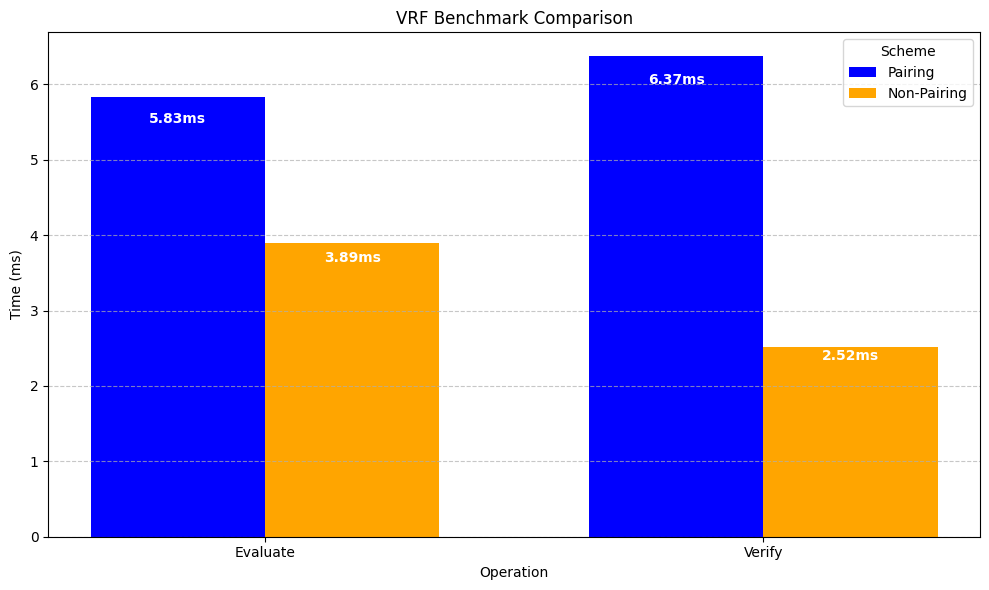
\includegraphics[width=0.75\linewidth]{figures/vrf-benchmark.png}
    \caption{VRF Benchmark}
    \label{fig:vrf-benchmark}
\end{figure}


Include benchmark of my construction on a different curve e.g. secpk251
Try to benchmark it against a VRF from the standardisation






% \subsection{CRBN Instantiation In Identity System}

% The Credential Relationship Binding Nullifier (CRBN) extends the Multi-Issuer Multi-Credential Anonymous Credential (MIMC-ABC) system from Chapter 3 to support a hierarchical structure with sybil resistance. We define two credential types: a \emph{Master Credential} containing a secret key $\k$, and \emph{Context Credentials} with context identifiers $\ctx$. A nullifier $\nul = g^{1/(\k + \ctx)} \in \G$ binds each Context Credential to the Master Credential, ensuring uniqueness per context while preserving privacy via zero-knowledge proofs.

% We modify MIMC-ABC’s algorithms as follows, reusing its position-binding Pedersen commitments and $\Sigma$-protocols. Let $\mathsf{pp}$ include $\G$, $p$, $g$, and commitment generators $(g_1, g_2, g_3, g_4, g)$, where $\ell = 4$ supports attributes $[\id, \ctx, \exp, \k]$ (extensible to more).

% \begin{itemize}
%     \item \textbf{Master Credential Issuance}:
%     \begin{itemize}
%         \item \emph{User}: Samples $\k \sample \Z_p$ and $\usk_m \sample \Z_p$. Computes commitment $\cmm = g_1^\id g_2^{\ctx_m} g_3^{\exp_m} g_4^\k g^{\usk_m}$, where $\ctx_m = \mathcal{H}(\text{"master"})$ and $\exp_m$ is the expiration. Runs $\mathsf{Obtain}(\attrs_m = [\id, \ctx_m, \exp_m, \k], \{\mathsf{opk}_j\}, \usk_m)$ with issuer $j_m$, proving $\cmm$’s opening via $\pircom$ (Section 2.4.3).
%         \item \emph{Issuer $j_m$}: Verifies the proof, signs $\sigma_m = \mathsf{RS.Sign}(\cmm, \mathsf{osk}_{j_m})$, and returns $\credm = (\sigma_m, \cmm)$ via $\mathsf{Issue}$.
%     \end{itemize}

%     \item \textbf{Context Credential Issuance}:
%     \begin{itemize}
%         \item \emph{User}: For context $\ctx_c$ (e.g., $\mathcal{H}(\text{"DMV"})$), samples $\usk_c \sample \Z_p$. Computes $\cmc = g_1^\id g_2^{\ctx_c} g_3^{\exp_c} g^{\usk_c}$ (no $\k$ here, as it’s from $\credm$). Runs $\mathsf{Obtain}(\attrs_c = [\id, \ctx_c, \exp_c, 0], \{\mathsf{opk}_j\}, \usk_c)$ with issuer $j_c$, proving $\cmc$’s opening and that position 4 is 0.
%         \item \emph{Issuer $j_c$}: Verifies the proof, optionally checks a nullifier registry (see below), signs $\sigma_c = \mathsf{RS.Sign}(\cmc, \mathsf{osk}_{j_c})$, and returns $\credc = (\sigma_c, \cmc)$.
%     \end{itemize}

%     \item \textbf{Nullifier Generation}: Given $\credm$ with $\k$ and $\credc$ with $\ctx_c$, compute:
%     \[
%     \nul = g^{1/(\k + \ctx_c)} \in \G
%     \]
%     where $\k + \ctx_c$ is computed in $\Z_p$, and the inverse $1/(\k + \ctx_c)$ exists with overwhelming probability (as $p$ is prime).

%     \item \textbf{Presentation and Verification}:
%     \begin{itemize}
%         \item \emph{User}: Inputs $\credm$, $\credc$, $\usk_m$, $\usk_c$, and a predicate $\phi$ (e.g., $\ctx_c = \text{"DMV"} \land \exp_c > \text{today}$). Rerandomizes $\credm$ to $(\sigma_m', \cmm')$ and $\credc$ to $(\sigma_c', \cmc')$ using $\Delta_{r_m}, \Delta_{r_c}$ (Section 3.3). Computes $\nul = g^{1/(\k + \ctx_c)}$ and proves:
%         \[
%         \mathcal{R}_{\mathsf{vrf}} = \zkpok \left\{ 
%         (\cmm', \cmc', \nul), (\id, \ctx_m, \exp_m, \k, \usk_m', \ctx_c, \exp_c, \usk_c') 
%         \middle|
%         \begin{array}{l}
%         \cmm' = g_1^\id g_2^{\ctx_m} g_3^{\exp_m} g_4^\k g^{\usk_m'} \land \ctx_m = \mathcal{H}(\text{"master"}) \land \\
%         \mathsf{RS.Ver}(\sigma_m', \cmm', \mathsf{opk}_{j_m}) = 1 \land \\
%         \cmc' = g_1^\id g_2^{\ctx_c} g_3^{\exp_c} g^{\usk_c'} \land \\
%         \mathsf{RS.Ver}(\sigma_c', \cmc', \mathsf{opk}_{j_c}) = 1 \land \\
%         \nul = g^{1/(\k + \ctx_c)} \land \phi(\ctx_c, \exp_c) = 1
%         \end{array} 
%         \right\}
%         \]
%         where $\usk_m' = \usk_m + \Delta_{r_m}$, $\usk_c' = \usk_c + \Delta_{r_c}$. The proof uses the $\Sigma$-protocol from Section 4.x (to be detailed).
%         \item \emph{Verifier}: Checks $\pi$, $\sigma_m'$, $\sigma_c'$, and $\nul$ against $\mathsf{opk}_{j_m}$, $\mathsf{opk}_{j_c}$. Optionally queries a nullifier registry to ensure $\nul$ is unused for $\ctx_c$.
%     \end{itemize}
% \end{itemize}

% \textbf{Note on Revocation}: If $\credm$ is revoked (e.g., via a public revocation list for $\cmm$ or $\k$), verifiers can reject proofs involving $\nul$, as $\k$’s validity underpins $\mathcal{R}_{\mathsf{vrf}}$. Details are deferred to Section 4.y.

% \textbf{Note on Sybil Resistance}: Issuers or verifiers may maintain a context-specific nullifier registry. During issuance, users prove $\nul$’s correctness in zero-knowledge; issuers reject duplicates. Alternatively, verifiers check $\nul$’s uniqueness during presentation, balancing privacy and accountability (see Section 4.z).

% This construction leverages MIMC-ABC’s efficient $\Sigma$-protocols and avoids pairings, using only standard group operations in $\G$. The nullifier $\nul$ enforces hierarchical binding and sybil resistance, computed deterministically from $\k$ and $\ctx_c$.





% \begin{table}
% \begin{center}
% \caption{Comparison of our construction over previous work.}
% \label{tab:comparison-chap4}
% \begin{tabular}{l|ccccc}
% Features    									& 
% Sybil Resist.  & 
% Hierarchy & 
% Private & 
% Pairing-Free & 
% Predicate Proofs \\
% \hline
% CanDID \cite{maram2021candid}     				&
% \ding{51}     & 
% \ding{51} 	& 
% \ding{55}  &  
% -     & 
% \ding{55}		\\
% SyRA \cite{crites_syra_2024}     				& 
% \ding{51}    	& 
% \ding{51}     & 
% \ding{51}  &  
% \ding{51}     & 
% \ding{55}		\\
% S3ID \cite{rabaninejad_attribute-based_2024}  & 
% \ding{51}     & 
% \ding{51}    	& 
% \ding{55}  &  
% \ding{55}     & 
% \ding{55}		\\
% UTT               & 
% \ding{51}     & 
% \ding{51}    	& 
% \ding{51}  &  
% \ding{55}     & 
% \ding{51}		\\
% Chap3             & 
% \ding{55}     & 
% \ding{55}    	& 
% \ding{51}  &  
% \ding{55}     & 
% \ding{51}		\\
% Ours  										& 
% \ding{51}     & 
% \ding{51}    	& 
% \ding{51}  &  
% \ding{51}     & 
% \ding{51}		\\
% \end{tabular}
% \end{center}
% \vspace{1em}
% \footnotetext[1]{Predicate Proofs allow users to prove statements about their credentials privately}
% \footnotetext[2]{Efficient Token refers to optimization of token verification}
% \end{table}


\subsection*{Notation}
Inline with our Anonymous Credential scheme built and prior chapters, the secret key is $\k$, the VRF input is $\ctx$, the VRF output is $\nul$ and the proof $\pi$ proves the correctness of $\nul$ such that $(\nul, \pi) \gets \mathsf{VRF.Eval}(\k, \ctx)$. $\cm = \CMCom([\id,\ldots];\usk)$ is a commitment shorthand for commitment $g_1^\id \ldots g^\usk$. We use Type-3 Bilinear Pairings. Let $\G_1$, $\G_2$, and $\G_T$ be groups of prime order $p$, with generators $g \in \G_1$, $\tilde{g} \in \G_2$, and a bilinear map $e: \G_1 \times \G_2 \to \G_T$.


\section{On the possibility of Sigma protocols for VRF Construction}
Why $\Sigma$-Protocols Suit Our VRF Construction

In our Verifiable Random Function (VRF) construction, we employ a $\Sigma$-protocol to generate the proof $\pi$ for the output $y = f_{sk}(x)$, where $sk$ is the secret key and $x$ is the input. A potential concern is whether the zero-knowledge property of $\Sigma$-protocols, which allows proof simulation, compromises the \textbf{verifiable uniqueness} property of the VRF—i.e., the guarantee that only one $y$ can be verified for a given $x$. Here, we explain why this concern is unfounded and how $\Sigma$-protocols align with VRF security requirements.

A VRF must satisfy three core properties: \textbf{correctness}, \textbf{uniqueness}, and \textbf{pseudorandomness}. \textbf{Correctness} ensures that an honestly computed output $y = f_{sk}(x)$ and its proof $\pi$ will always pass verification. \textbf{Uniqueness} guarantees that for each $x$, only one $y$ can be successfully verified with a proof $\pi$. \textbf{Pseudorandomness} ensures that without $sk$, $y$ is indistinguishable from random, even after seeing other $(x, y, \pi)$ triples. The $\Sigma$-protocol, an interactive proof system, offers three key properties: \textbf{completeness} (an honest prover with $sk$ convinces the verifier), \textbf{soundness} (a dishonest prover cannot prove a false statement), and \textbf{zero-knowledge} (the proof reveals nothing about $sk$, and a simulator can mimic it for true statements). These align perfectly with the VRF's needs: completeness supports correctness, soundness enforces uniqueness, and zero-knowledge preserves pseudorandomness by hiding $sk$.

The zero-knowledge property ensures $sk$ remains secret, but the simulator can only generate valid proofs for \textbf{true statements}, e.g., $y = f_{sk}(x)$. It cannot produce a proof for a false statement, like $y' \neq f_{sk}(x)$, that passes verification, due to the \textbf{soundness} property. Soundness ensures that only proofs for the correct $y$ are accepted, preventing an adversary from forging a proof for an incorrect output. Thus, the uniqueness of $y$ is preserved, as false proofs are rejected with overwhelming probability.

\textbf{Concrete Example:} Consider a VRF where $y = g^{1/(sk + x)}$ in a group of prime order $p$, and the $\Sigma$-protocol proves $y^{sk + x} = g$. Here, $y$ is uniquely determined by $sk$ and $x$ (since exponentiation is injective for $sk + x \neq 0 \mod p$). The $\Sigma$-protocol ensures that only the correct $y$ satisfies the equation, and a proof for an incorrect $y'$ (where $y'^{sk + x} \neq g$) fails verification. Despite zero-knowledge allowing simulation for the true $y$, soundness prevents valid proofs for false $y'$, reinforcing uniqueness.

A potential concern with using zero-knowledge proofs for VRFs is that proof simulatability might conflict with output uniqueness. In general NIZKs, the simulation property could potentially allow valid proofs for multiple outputs of the same input, e.g. $y_1, y_2$ for the same input $x$, violating the VRF uniqueness requirement. Our construction resolves this tension by leveraging a $\Sigma$-protocol to prove the statement $y^{sk + x} = g$ where $y = g^{1/(sk + x)}$. This equation has exactly one solution for $y$ given fixed values of $sk$ and $x$ (when $sk + x \neq 0 \mod p$). While the protocol's zero-knowledge property conceals $sk$, its soundness guarantees that only proofs for the correct $y$ will verify, thereby enforcing rather than compromising uniqueness.


In conclusion, the zero-knowledge property of $\Sigma$-protocols does not weaken the VRF's verifiable uniqueness, as simulation is limited to true statements. Meanwhile, soundness upholds the integrity of the proof, ensuring only the correct $y$ verifies.